% !TEX root =../main.tex

\chapter{Einleitung}


\section{Anwendungsfall}

Beim Online-Shopping kann es leicht passieren, dass der Käufer bezüglich seiner Kaufentscheidung unschlüssig ist. Es fällt dem Käufer schwer ein Produkt auszuwählen. Einer der Hauptgründe hierfür, ist laut Meinung der Autorin, eine unzureichende Informationslage während des Kaufprozesses. Der Kunde ist so vielleicht nicht in der Lage ein geeignetes Produkt zu finden oder ist nicht in der Lage aus geeigneten Alternativen ein Produkt auszuwählen. Fehlende Vorschläge oder Beratung können dazu führen, dass der Kaufprozess in einer solchen Situation abgebrochen wird.

% TODO: Bitte prüfen, ob das folgende Zitat vollständig ist. Es sieht so aus, als ob das Ende des letzten Satzes fehlt.

\begin{description}
\item[Unzureichende Informationen] Wenn Käufer und Verkäufer nicht den gleichen Informationsstand besitzen, wird dies laut \textcite{akerlof:lemons} als \term{asymmetrische Information} bezeichnet und wie folgt definiert: \glqq Asymmetrische Information, bezeichnet den Zustand, in dem zwei Vertragsparteien bei Abschluss und/oder Erfüllung eines Vertrags oder Marktteilnehmer nicht über dieselben Information verfügen. Die Auseinandersetzung mit Problemen, die aus asymmetrischen Informationen resultieren\grqq
\end{description}

Ein Beispiel für asymmetrische Information kann z. B. beim Kauf eines Autos vorliegen. Nicht jeder Käufer besitzt detaillierte Kenntnisse über Ausstattungsdetails, Motor oder Getriebe der zum Verkauf angebotenen Autos. Auf der Gegenseite besitzen die Verkäufer weitreichende Kenntnisse über die von ihnen verkauften Autos und könnten sich sogar, aus Gründen der Gewinnmaximierung, in einem Interessenkonflikt befinden, der eine objektive Beratung beeinflusst. In diesem Fall ist für den Käufer die Beratung durch einen Freund wünschenswert, welcher fundierte Kenntnisse in diesem Bereich besitzt.


Aus diesem Grund ist kooperatives Einkaufen besonders geeignet um den Kauf von wertvollen, spezialisierten und fachlichen Produkten wie Computern, Häusern, Kameras u. v. m. zu unterstützen.

\begin{description}
\item[Fehlende Erfahrung] Bei dem Kauf mancher Produkte oder Dienstleistungen, sind nur geringe Vorkenntnisse nötig. Beispielsweise für das Buchen einer Reise. Man benötigt mehrere Informationen und Tipps für den gewünschten Urlaubsort. Die Erfahrungen und Bewertungen von anderen Leuten sind hilfreich.
\item[Finanzierung, (Pay by Others)] Wenn ein Käufer nicht für die ausgewählten Produkte bezahlen kann, möchte er vielleicht die finanzielle Überstützung eines Bekannten oder Freundes in Anspruch nehmen.
\end{description}


\section{Motivation}

Soziale Netzwerke erfreuen sich großer Beliebtheit und ihre Betreiber zählen zu den größten Internetunternehmen der Welt. Laut \textcite{sokolov:facebook} kann das soziale Netzwerk Facebook bereits 2 Milliarden Nutzer vorweisen. In einer durch \textcite{nasdaq} aufgestellten Statistik belegt Facebook den 5. Platz der größten Internetunternehmen, gemessen an ihrem Börsenwert. \textcite{mittermeier} listet Facebook gar auf dem dritten Platz. Es ist anzumerken, dass in beiden Statistiken Facebook direkt hinter dem Online-Versandhändler Amazon gelistet wird. Am Börsenwert gemessen scheint der Online-Handel die sozialen Netzwerke sogar noch zu überflügeln. Es scheint zumindest sicher, dass sowohl soziale Netzwerke als auch Web-Shops sich eines großen Erfolgs erfreuen.

Die Motivation hinter dem Erstellen dieser Arbeit ist, herauszuarbeiten wie soziale Netzwerke mit Webshops verbunden werden können, um so Synergien zwischen zwei der populärsten Arten von Webapplikation zu ermöglichen.

Das Anwendungsfalldiagramm \vref{fig:online-shopping} zeigt, wie Anwendungsfälle aus sozialen Netzwerken und Webshops verbunden werden können:

\begin{figure}[htbp]
	\centering
	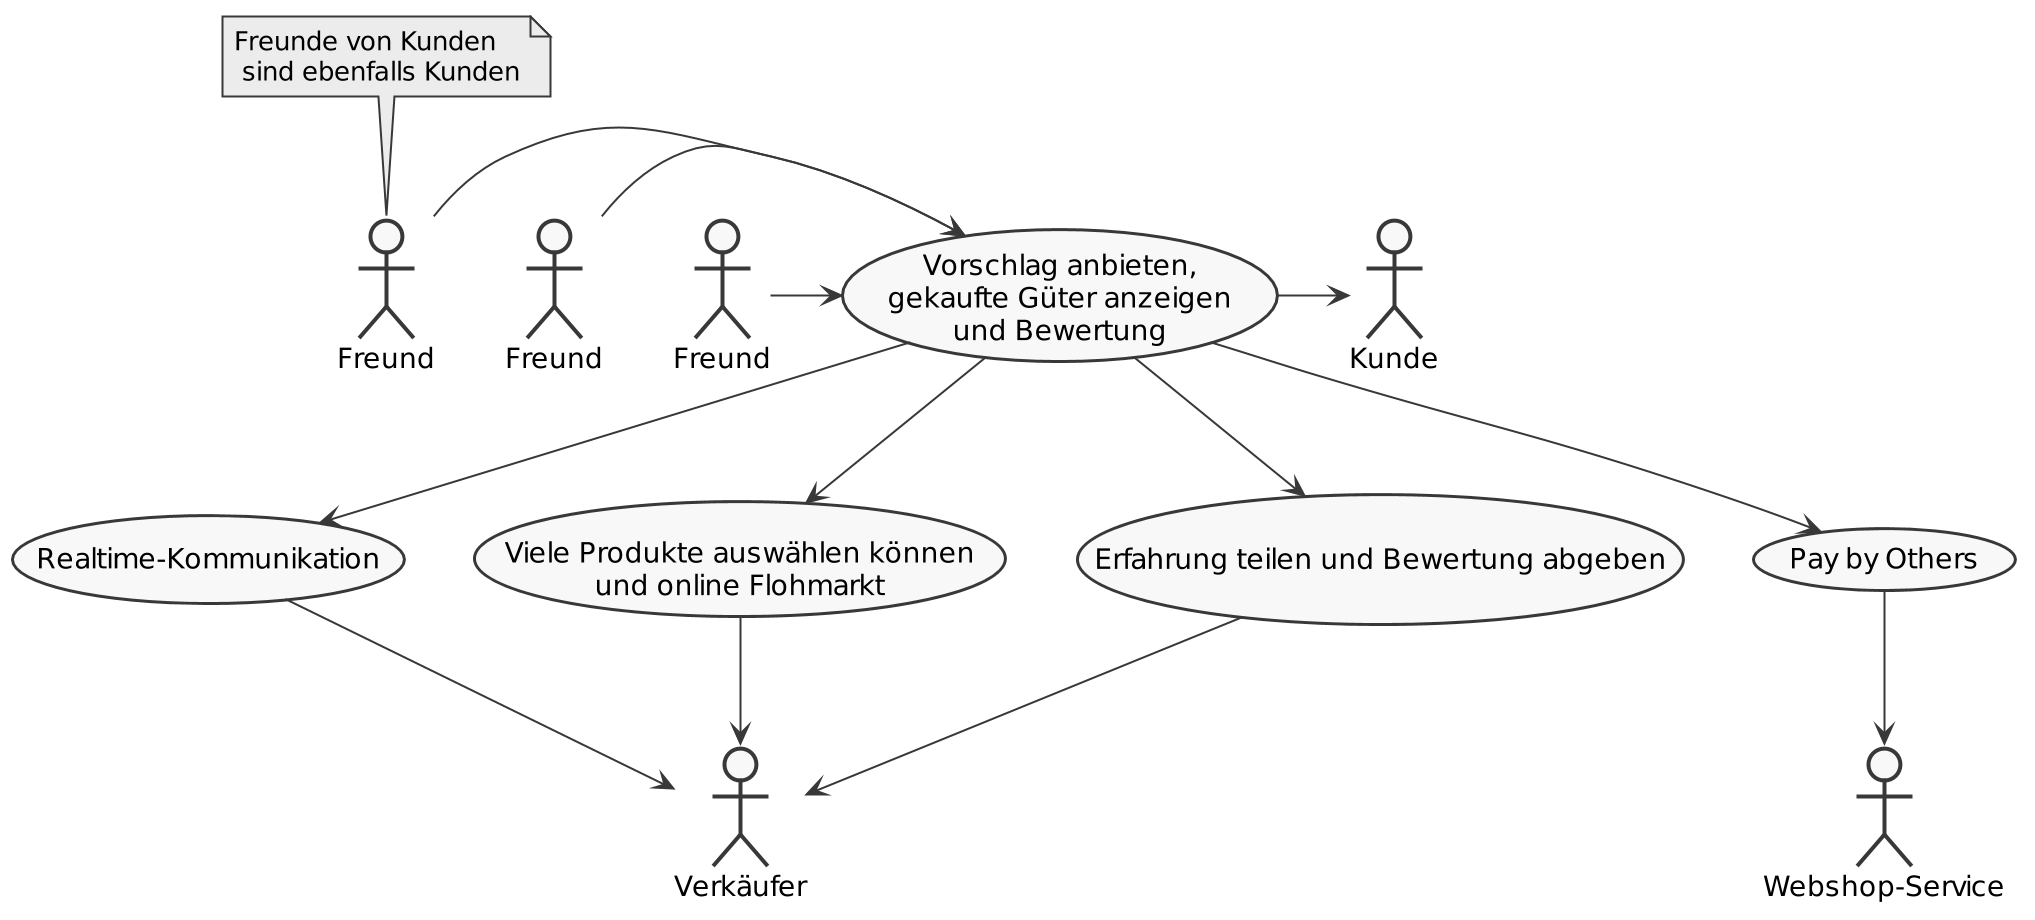
\includegraphics[width=0.7\textwidth]{uml-diagramme/online-shopping.png}
	\caption{Online Shopping}
	\label{fig:online-shopping}
\end{figure}


\subsection{Zielstellung}

Ziel dieser Arbeit ist herauszuarbeiten, wie Webshops mit Sozialen Netzwerken kombiniert werden können?

Im Rahmen dieser Arbeit sollen die Konzepte und Mechanismen der meistgenutzten Webshops mit einer Auswahl an Social-Media-Angeboten untersucht und verglichen werden. Es soll untersucht werden, welche unterschiedlichen Geschäftsmodelle zum Einsatz kommen und wie diese kombiniert werden können. Abschließend soll ein Konzept eines Webshops entwickelt werden, der Konzepte von Social-Media-Webseiten mit denen eines Webshops vereint. Dieses Konzept soll Möglichkeiten aufzeigen, wie in einem Webshop die Tätigkeit des Einkaufens mit anderen Nutzern geteilt und kooperativ erlebt werden kann.

Die Kooperation soll hierbei komplett in der konzeptionierten Webapplikation abgebildet werden. Es sollen keine Zusätzlichen Kommunikationskanäle notwendig sein.

Innerhalb dieser Bachelorarbeit soll darüber hinaus die These untersucht werden, das Kooperation in Webshops im Stil von online Computerspielen abgebildet werden kann.


\section{Methoden}

Die Bachelorarbeit beginnt damit, die Konzepte von E-Commerce, Social Media und Social Commerce zu betrachten. Anschließend wird untersucht wie im Bereich des Online Gamings eine Kooperation von Nutzern ermöglicht und gefördert wird. Darauf folgend werden Anwendungsfälle definiert, welche ein Webshop unterstützen muss, um kooperatives Einkaufen zu ermöglichen. Auf der Basis dieser Anwendungsfälle wird eine Untermenge der Untersuchten Konzepte ausgewählt und ein Entwurf eines Prototyps angefertigt.

Die Bachelorarbeit schließt mit der Betrachtung dieses Entwurfs ab. Es werden offene Punkte dargelegt und es wird ein Fazit gezogen.


\section{Artefakte}

Bei dem konzipierten Webshop können Kunden kooperativ einkaufen. Vorschläge und Beratung durch andere Nutzer zu bekommen, ist in die Applikation integriert. Der Kunde benötigt hierfür keine zusätzlichen Anwendungen.


\section{Abgrenzung}

Innerhalb dieser Arbeit werden keine technische Probleme wie Performanz oder Datensicherheit der Applikation untersucht. Auch die Skalierung der Anwendung auf verteilte Systeme oder die \term{Cloud} wird nicht betrachtet.
